\documentclass[11pt]{article}

\usepackage[sc]{mathpazo} % math & rm
\linespread{1.05}        % Palatino needs more leading (space between lines)
\usepackage[scaled=0.90]{helvet} % ss
\usepackage[scaled=0.85]{beramono} % tt
\usepackage[T1]{fontenc}
\usepackage{textcomp}
\usepackage{varwidth}

\usepackage{amsmath}
\usepackage{amssymb}
\usepackage{amsthm}
\usepackage{bm}
\usepackage{graphicx}
\usepackage{float}
\providecommand{\abs}[1]{\lvert#1\rvert}
\providecommand{\norm}[1]{\lVert#1\rVert}


\newtheorem{thm}{Theorem}
\newtheorem{lemma}[thm]{Lemma}
\newtheorem{fact}[thm]{Fact}
\newtheorem{cor}[thm]{Corollary}
\newtheorem{eg}{Example}
\newtheorem{ex}{Exercise}
\newtheorem{defi}{Definition}
\newtheorem{hw}{Problem}
\newenvironment{sol}
{\par\vspace{3mm}\noindent{\it Solution}.}
{\qed}

\newcommand{\ov}{\overline}
\newcommand{\cb}{{\cal B}}
\newcommand{\cc}{{\cal C}}
\newcommand{\cd}{{\cal D}}
\newcommand{\ce}{{\cal E}}
\newcommand{\cf}{{\cal F}}
\newcommand{\ch}{{\cal H}}
\newcommand{\cl}{{\cal L}}
\newcommand{\cm}{{\cal M}}
\newcommand{\cp}{{\cal P}}
\newcommand{\cz}{{\cal Z}}
\newcommand{\eps}{\varepsilon}
\newcommand{\ra}{\rightarrow}
\newcommand{\la}{\leftarrow}
\newcommand{\Ra}{\Rightarrow}
\newcommand{\dist}{\mbox{\rm dist}}
\newcommand{\bn}{{\mathbf N}}
\newcommand{\bz}{{\mathbf Z}}
\newcommand{\bbR}{{\mathbb R}}

\newcommand{\pder}[2][]{\frac{\partial#1}{\partial#2}}
\newcommand{\omitJ}{(\bm{\cdot})}
\newcommand{\pderJ}[1]{\pder[\omitJ]{#1}}
\setlength{\parindent}{0pt}
% \setlength{\parskip}{2ex}
\newenvironment{proofof}[1]{\bigskip\noindent{\itshape #1. }}{\hfill$\Box$\medskip}

\usepackage{enumerate,fullpage,proof,color}

\title{CS224N: Assignment \#1}
\author{Kangwei Ling}

\begin{document}
\maketitle

\section{Softmax}
\label{sec:1}

\begin{enumerate}[(a)]
\item eliminate the term $c$.
  \[
    softmax(\bm{x + c})_i = \dfrac{e^{\bm{x}_i + c}}{\sum_je^{\bm{x}_j + c}} =
    \dfrac{e^c\cdot e^{\bm{x}_i}}{e^c\cdot \sum_je^{\bm{x}_j}} = softmax(\bm{x})_i 
  \]
\item in \verb|q1_softmax.py|.
\end{enumerate}

\section{Neural Network Basics}
\label{sec:2}

\begin{enumerate}[(a)]
\item \
  \[
    \frac{d}{dx}\sigma(x) = \frac{-1}{(1 + e^{-x})^2}\cdot (e^{-x})' =
    \frac{-1}{(1 + e^{-x})^2}\cdot ( - e^{-x}) = \frac{1}{1 + e^{-x}} \cdot
    \frac{e^{-x}}{1 + e^{-x}} = \sigma(x)(1 - \sigma(x))
  \]
\item As $\bm{y}$ is the one-hot label vector, $\sum_jy_j = 1$, 
  and
  \begin{align*}
    \frac{\partial \hat{y}_j}{\partial \theta_i} =
    \begin{cases}
      -\hat{y}_j\hat{y}_i  &\ \mbox{if } i \neq j \\
      \hat{y}_j(1 - \hat{y}_j) &\ \mbox{otherwise} 
    \end{cases}
  \end{align*}
  thus
  \begin{align*}
    \frac{\partial }{\partial\theta_i}CE(\bm{y}, \hat{\bm{y}}) &= - y_i(1 - \hat{y}_i) - \sum_{j \neq i} y_j (- \hat{y}_i) \\
                                                               &= -y_i + y_i\hat{y}_i + \hat{y}_i\sum_{j \neq i} y_j \\
                                                               &= \hat{y}_i\sum_{j} y_j - y_i \\
    &= \hat{y}_i - y_i
  \end{align*}
  Therefore, $\dfrac{\partial}{\partial \theta}CE(\bm{y}, \hat{\bm{y}}) = \hat{\bm{y}}
  - \bm{y}$.
\item First find the gradients with respect to the hidden layer $\bm{h}$. Let
  $\bm{z_2} = \bm{hW}_2 + \bm{b}_2, \bm{z_1} = \bm{xW}_1 + \bm{b}_1,
  \bm{\delta}_2 = \pderJ{\bm{z_2}}, \bm{\delta}_1 = \pderJ{\bm{z_1}}$. ($(\cdot)
  = CE(\bm{y}, \hat{\bm{y}})$, $\circ$ means piecewise multiplication).
  thus
  \begin{align*}
    \bm{\delta}_2 &= \hat{\bm{y}} - \bm{y}  \\
    \pderJ{\bm{h}} &= \bm{\delta}_2\bm{W_2}^T \\
    \bm{\delta}_1 &= \bm{\delta}_2\bm{W_2}^T \circ \sigma'(\bm{z_1}) \\
    \bm{\delta}_3 &= \pderJ{\bm{x}} = \bm{\delta}_1\bm{W_1}^T
  \end{align*}
  
\item $D_xH + HD_y + H + D_y$
  
\item \verb|q2_sigmoid.py|
\item \verb|q2_gradcheck.py|
\item \verb|q2_neural.py|
\end{enumerate}

\section{word2vec}
\label{sec:3}

\begin{enumerate}[(a)]
\item Let $\bm{y}, \hat{\bm{y}}$ be column vectors. All vectors are column vectors.
  \[
    \pder[J]{\bm{v}_c} = \bm{U}(\hat{\bm{y}} - \bm{y})
  \]
  
\item \
  \[
    \pder[J]{\bm{u}_i} = (\hat{y}_i - y_i)\bm{v}_c
  \]
  \[
    \pder[J]{\bm{U}} = \bm{v}_c(\hat{\bm{y}} - \bm{y})^T
  \]
  
\item gradients with respect to $\bm{v}_c$:
  \begin{align*}
    \pder[J]{\bm{v}_c} = (\sigma(\bm{u}_o^T\bm{v}_c) - 1)\bm{u}_o + \sum_{k=1}^K (1 - \sigma(-\bm{u}_k^T\bm{v}_c))\bm{u}_k
  \end{align*}
  gradients with respect to $\bm{U}$:
  \begin{align*}
    \pder[J]{\bm{u}_i} =
    \begin{cases}
      (\sigma(\bm{u}_o^T\bm{v}_c) - 1)\bm{v}_c \ \ &\mbox{if } i = o \\
       (1 - \sigma(-\bm{u}_i^T\bm{v}_c))\bm{v}_c \ \ &\mbox{if } i \in \{1,\dots, K\} \\
      0 \ \ & \mbox{otherwise}
    \end{cases}
  \end{align*}
  
  
\item For skip-gram:
  \begin{align*}
    \pder[J_{skip-gram}]{\bm{U}} &= \sum_{-m \leq j\leq m, j\neq 0} \pder[F(\bm{w}_{c+j}, \bm{v}_c)]{\bm{U}} \\
    \pder[J_{skip-gram}]{\bm{v}_c} &= \sum_{-m \leq j\leq m, j\neq 0} \pder[F(\bm{w}_{c+j}, \bm{v}_c)]{\bm{v}_c} \\
    \pder[J_{skip-gram}]{\bm{v}_i} &= \bm{0} \ \ \text{ for } i \neq c\\
  \end{align*}
  For CBOW:
  \begin{align*}
    \pder[J_{CBOW}]{\bm{U}} &= \pder[F(\bm{w}_c, \hat{\bm{v}})]{\bm{U}} \\
    \pder[J_{CBOW}]{\bm{v}_{j}} &= \pder[F(\bm{w}_c, \hat{\bm{v}})]{\hat{\bm{v}}} \ \ \text{ for } j \in \{c-m, ..., c-1, c+1, ..., c+m \} \\
    \pder[J_{CBOW}]{\bm{v}_{j}} &= \bm{0} \ \ \text{ for } j \notin \{c-m, ..., c-1, c+1, ..., c+m \}
  \end{align*}
\item \verb|q3_word2vec.py|
\item \verb|q3_sgd.py|
\item \
  \begin{center}
    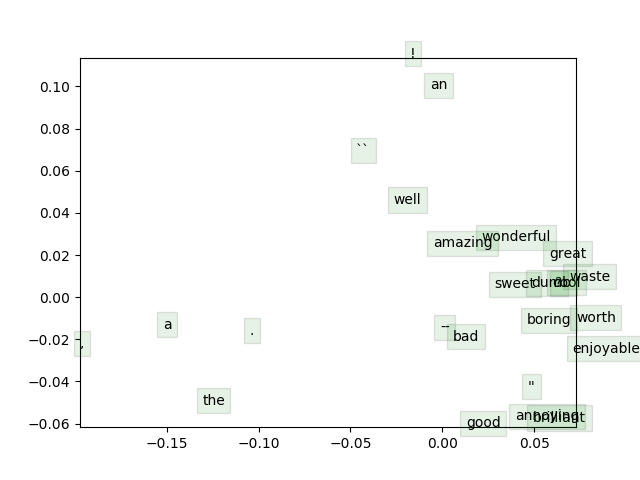
\includegraphics[scale=0.8]{../assignment1/q3_word_vectors.png}
  \end{center}
\item \verb|q3_word2vec.py|
\end{enumerate}

\section{Sentiment Analysis}
\label{sec:4}

\begin{enumerate}[(a)]
\item \verb|q4_sentiment.py|
\item To prevent out model from overfitting.
\item \verb|q4_sentiment.py|
\item \
  \begin{table}[H]
    \centering
    \begin{tabular}{|c|c|c|}
      \hline
      Best Accuracies& word vectors from problem 3& pretrained \\ \hline \hline
      train & 31.121& 39.934  \\ \hline
      dev & 32.698& 36.876\\ \hline
      test & 30.271& 37.69  \\ \hline
    \end{tabular}
    \caption{best accuracies}
    \label{tab:1}
  \end{table}
  The model using pretrained GloVe vectors outperforms for the following
  reasons:
  \begin{itemize}
  \item The word vectors are trained on massive data (wikipedia), thus hold more
    information
  \item GloVe's vectors use different dimension from word2vec.
  \item GloVe represents words better than word2vec.
  \end{itemize}
\item \ 
  \begin{center}
    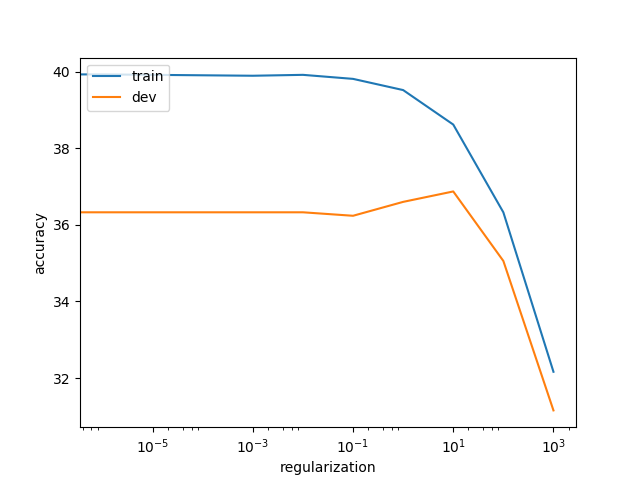
\includegraphics[scale=.8]{../assignment1/q4_reg_v_acc.png}
  \end{center}
  Regularization helped tackle overfitting, but regularization with too big
  weight harm the performance.
\item \ 
  \begin{center}
    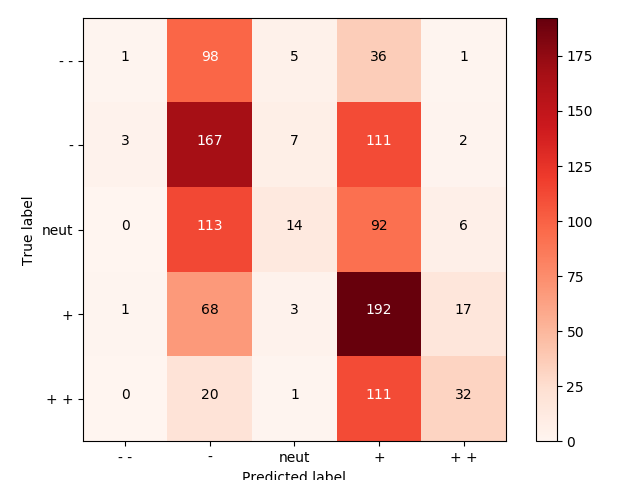
\includegraphics[scale=.8]{../assignment1/q4_dev_conf.png}
  \end{center}
  The mispredictions of the model mostly happened near neutral zone. For strong
  sentiment sentence, the prediction is quite accurate.
\item
  \begin{itemize}
  \item Some cold/negative words in the sentence cause the whole sentence to be
    predicted as negative, while the sentence has a positive context.(Or
    negative meaning get overrun with positive words)
    \begin{center}
      \begin{varwidth}{.7\textwidth}
    {\small nothing 's at stake , just a twisty double-cross you can smell a mile away -- still , the derivative nine queens is lots of fun .}              
      \end{varwidth}
    \end{center}
    This sentence is with positive label(3), yet was predicted as negative(1).
\item Some negation words are not exhibiting their negating effect.
    \begin{center}
      \begin{varwidth}{.7\textwidth}
    {\small scores no points for originality , wit , or intelligence .}             
  \end{varwidth}
    \end{center}
True label(0), predicted label(3).
    \item Names hurt performance.
    \begin{center} 
      \begin{varwidth}{.7\textwidth}
    {\small it takes a strange kind of laziness to waste the talents of robert forster , anne meara , eugene levy , and reginald veljohnson all in the same movie .}              
      \end{varwidth}
    \end{center}
    True label(0), predicted label(3).
  \end{itemize}
\end{enumerate}
\end{document}
